\chapter{Réalisation et Développement}

\section{Environnement de Développement}

\subsection{Outils et IDE}

L'environnement de développement a été soigneusement configuré pour maximiser la productivité et garantir la qualité du code produit. 

\begin{figure}[H]
\centering
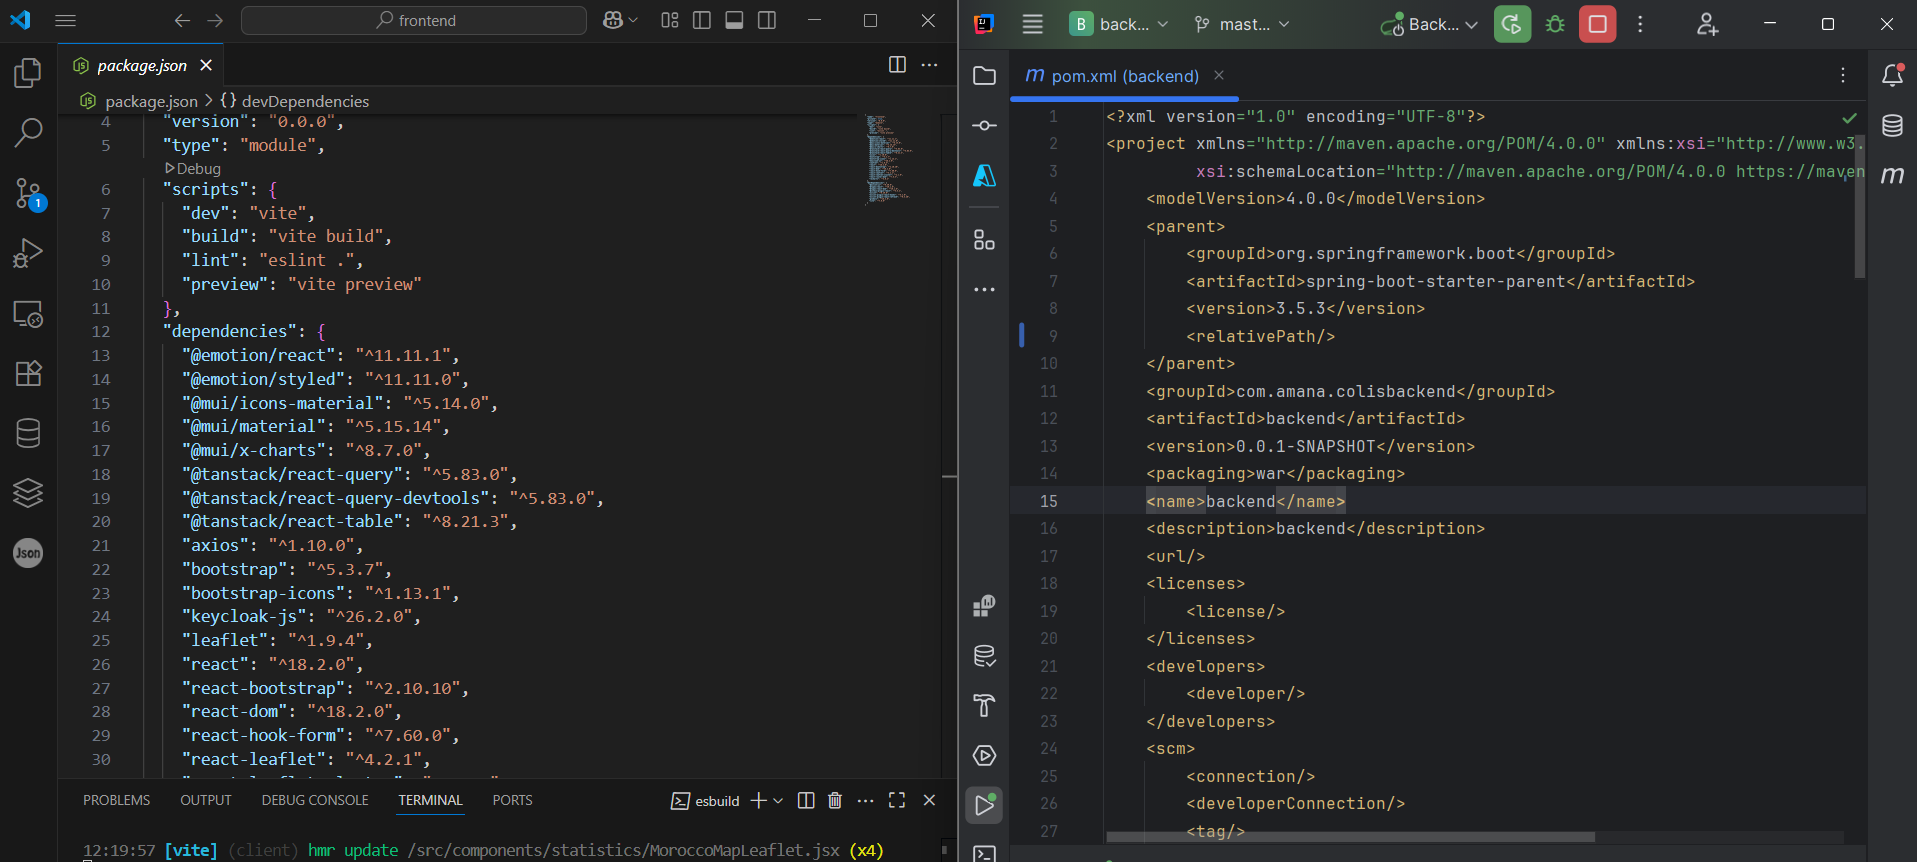
\includegraphics[width=1.0\textwidth]{images/dev_environment.png}
\caption{Environnement de développement complet}
\label{fig:dev_environment}
\end{figure}

La Figure \ref{fig:dev_environment} présente l'environnement de développement utilisé avec IntelliJ IDEA Ultimate pour le backend Spring Boot et Visual Studio Code pour le frontend React. IntelliJ IDEA [15] offre une intégration native excellente avec les frameworks Spring, des outils de débogage avancés, et un support complet de MongoDB. Visual Studio Code [16] a été choisi pour sa richesse d'extensions React et sa légèreté pour le développement frontend.

Git [17] a été configuré avec des hooks de pre-commit pour automatiser la vérification de la qualité du code. Docker [18] facilite la gestion des services externes (MongoDB, MySQL, Keycloak) avec des configurations prêtes à l'emploi, assurant la reproductibilité de l'environnement entre les différents postes de développement.

\subsection{Frameworks et bibliothèques}

\begin{figure}[H]
\centering
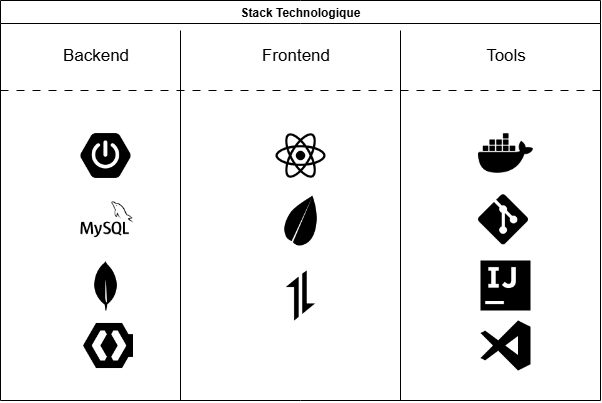
\includegraphics[width=0.8\textwidth]{images/tech_stack.png}
\caption{Stack technologique utilisée}
\label{fig:tech_stack}
\end{figure}

La Figure \ref{fig:tech_stack} illustre la stack technologique complète du projet. Le backend s'articule autour de Spring Boot 3.1 [1] avec Spring Data JPA [3] pour MySQL et Spring Data MongoDB [4] pour la base documentaire. Spring Security 6.1 [2] gère l'authentification OAuth2 [11,12] avec Keycloak [8]. Le frontend React 18.2 [5] exploite les dernières fonctionnalités de performance avec React Router [22] pour la navigation et Axios [21] pour les communications HTTP.

La cartographie utilise Leaflet [9] avec React-Leaflet [10], enrichie par Leaflet.markercluster [24] pour le clustering des points et des providers de tiles haute résolution. Cette combinaison offre des performances d'affichage optimales même avec des milliers de marqueurs simultanés.

\subsection{Configuration du projet}

\begin{figure}[H]
\centering
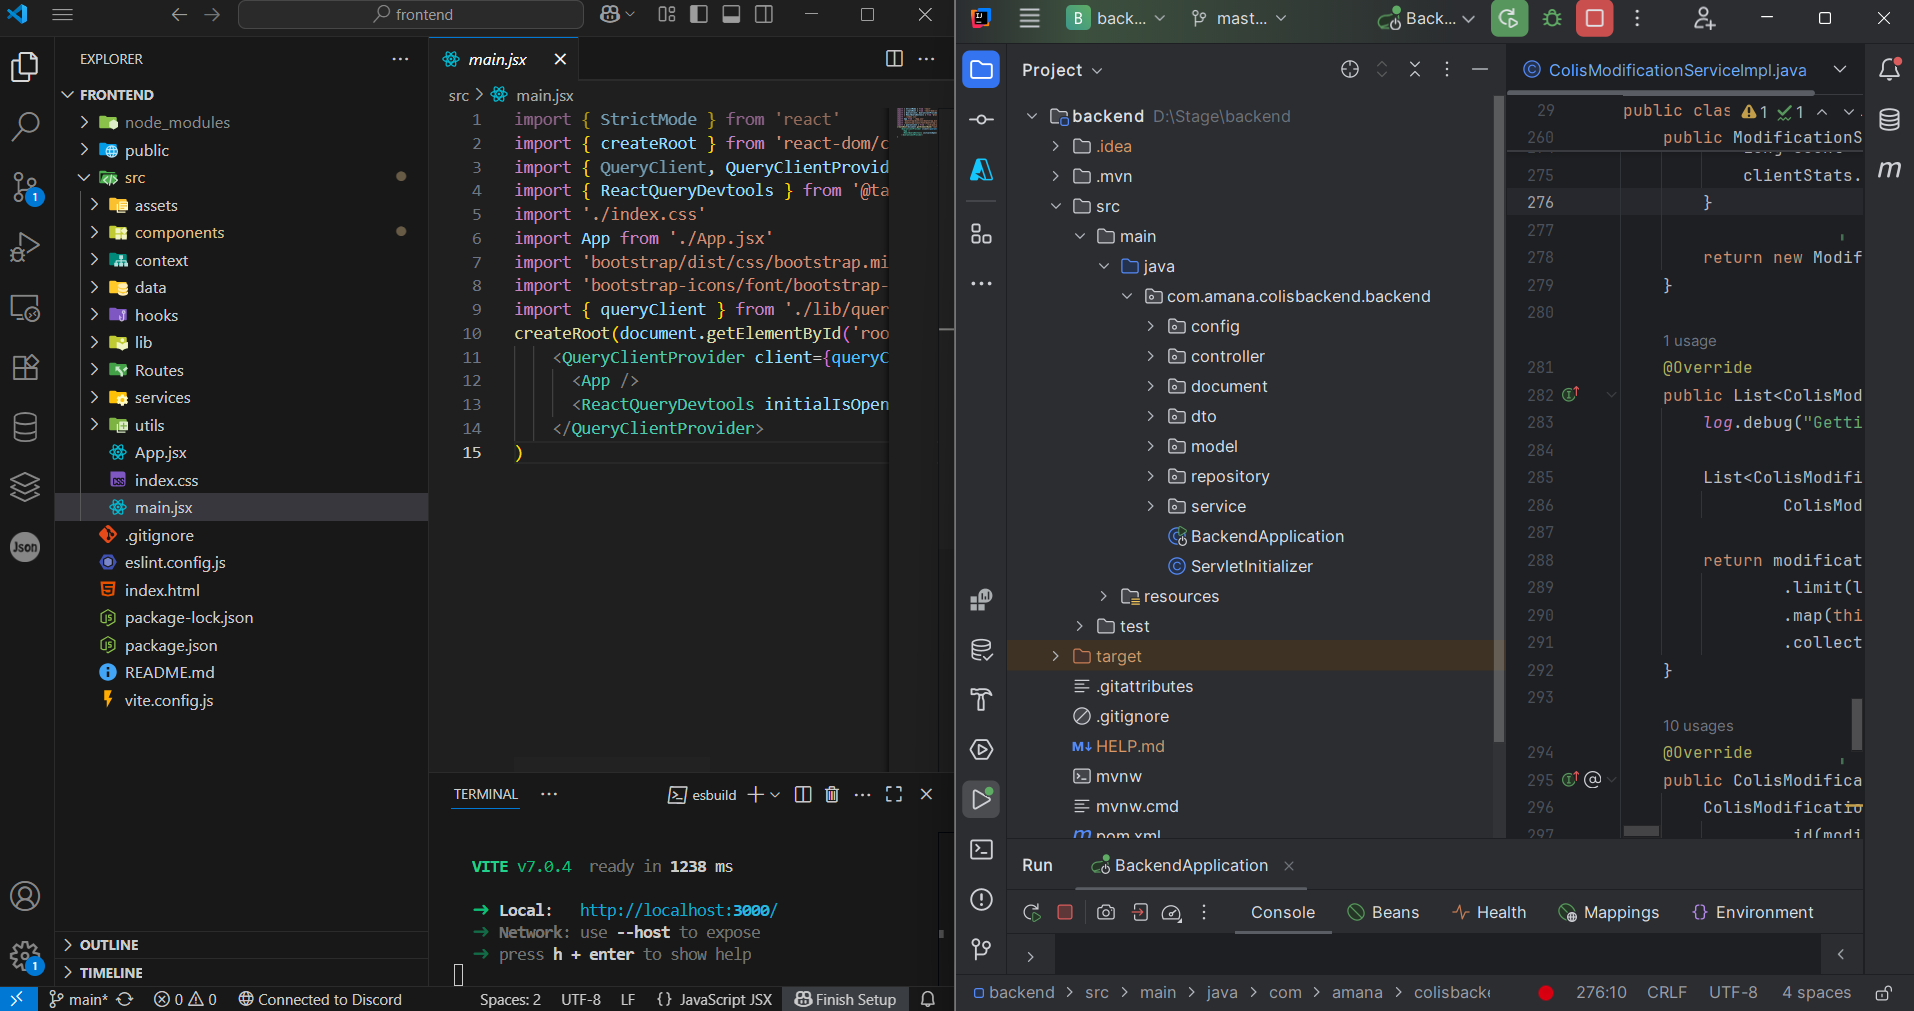
\includegraphics[width=0.8\textwidth]{images/project_structure.png}
\caption{Structure du projet et organisation des fichiers}
\label{fig:project_structure}
\end{figure}

La Figure \ref{fig:project_structure} montre l'organisation du projet respectant les bonnes pratiques d'architecture. Le backend adopte une organisation par feature plutôt que par couche technique, facilitant la maintenance. Le frontend suit la structure Create React App avec des dossiers organisés par fonctionnalité : components, services, hooks, utils.

\section{Développement Backend}

\subsection{Architecture Spring Boot}

\begin{figure}[H]
\centering
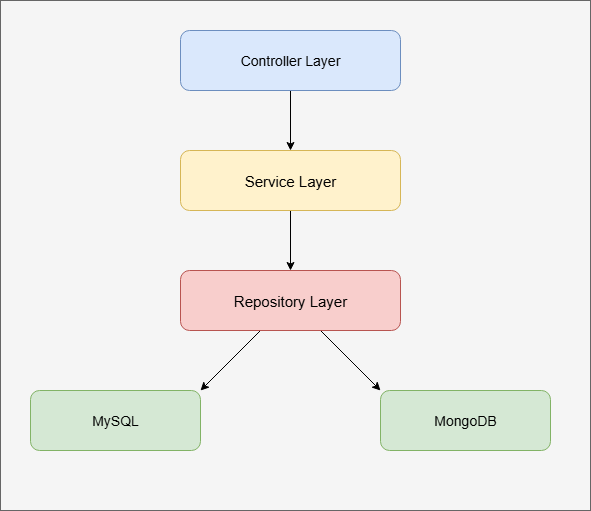
\includegraphics[width=0.5\textwidth]{images/spring_architecture.png}
\caption{Architecture Spring Boot avec couches séparées}
\label{fig:spring_architecture}
\end{figure}

La Figure \ref{fig:spring_architecture} illustre l'architecture backend implémentant le pattern Repository avec une couche de service métier orchestrant les interactions entre MySQL et MongoDB. La couche Controller expose les API REST, la couche Service implémente la logique métier, et la couche Repository abstrait l'accès aux données avec des implémentations spécialisées.

\subsection{Services et contrôleurs}

\begin{figure}[H]
\centering
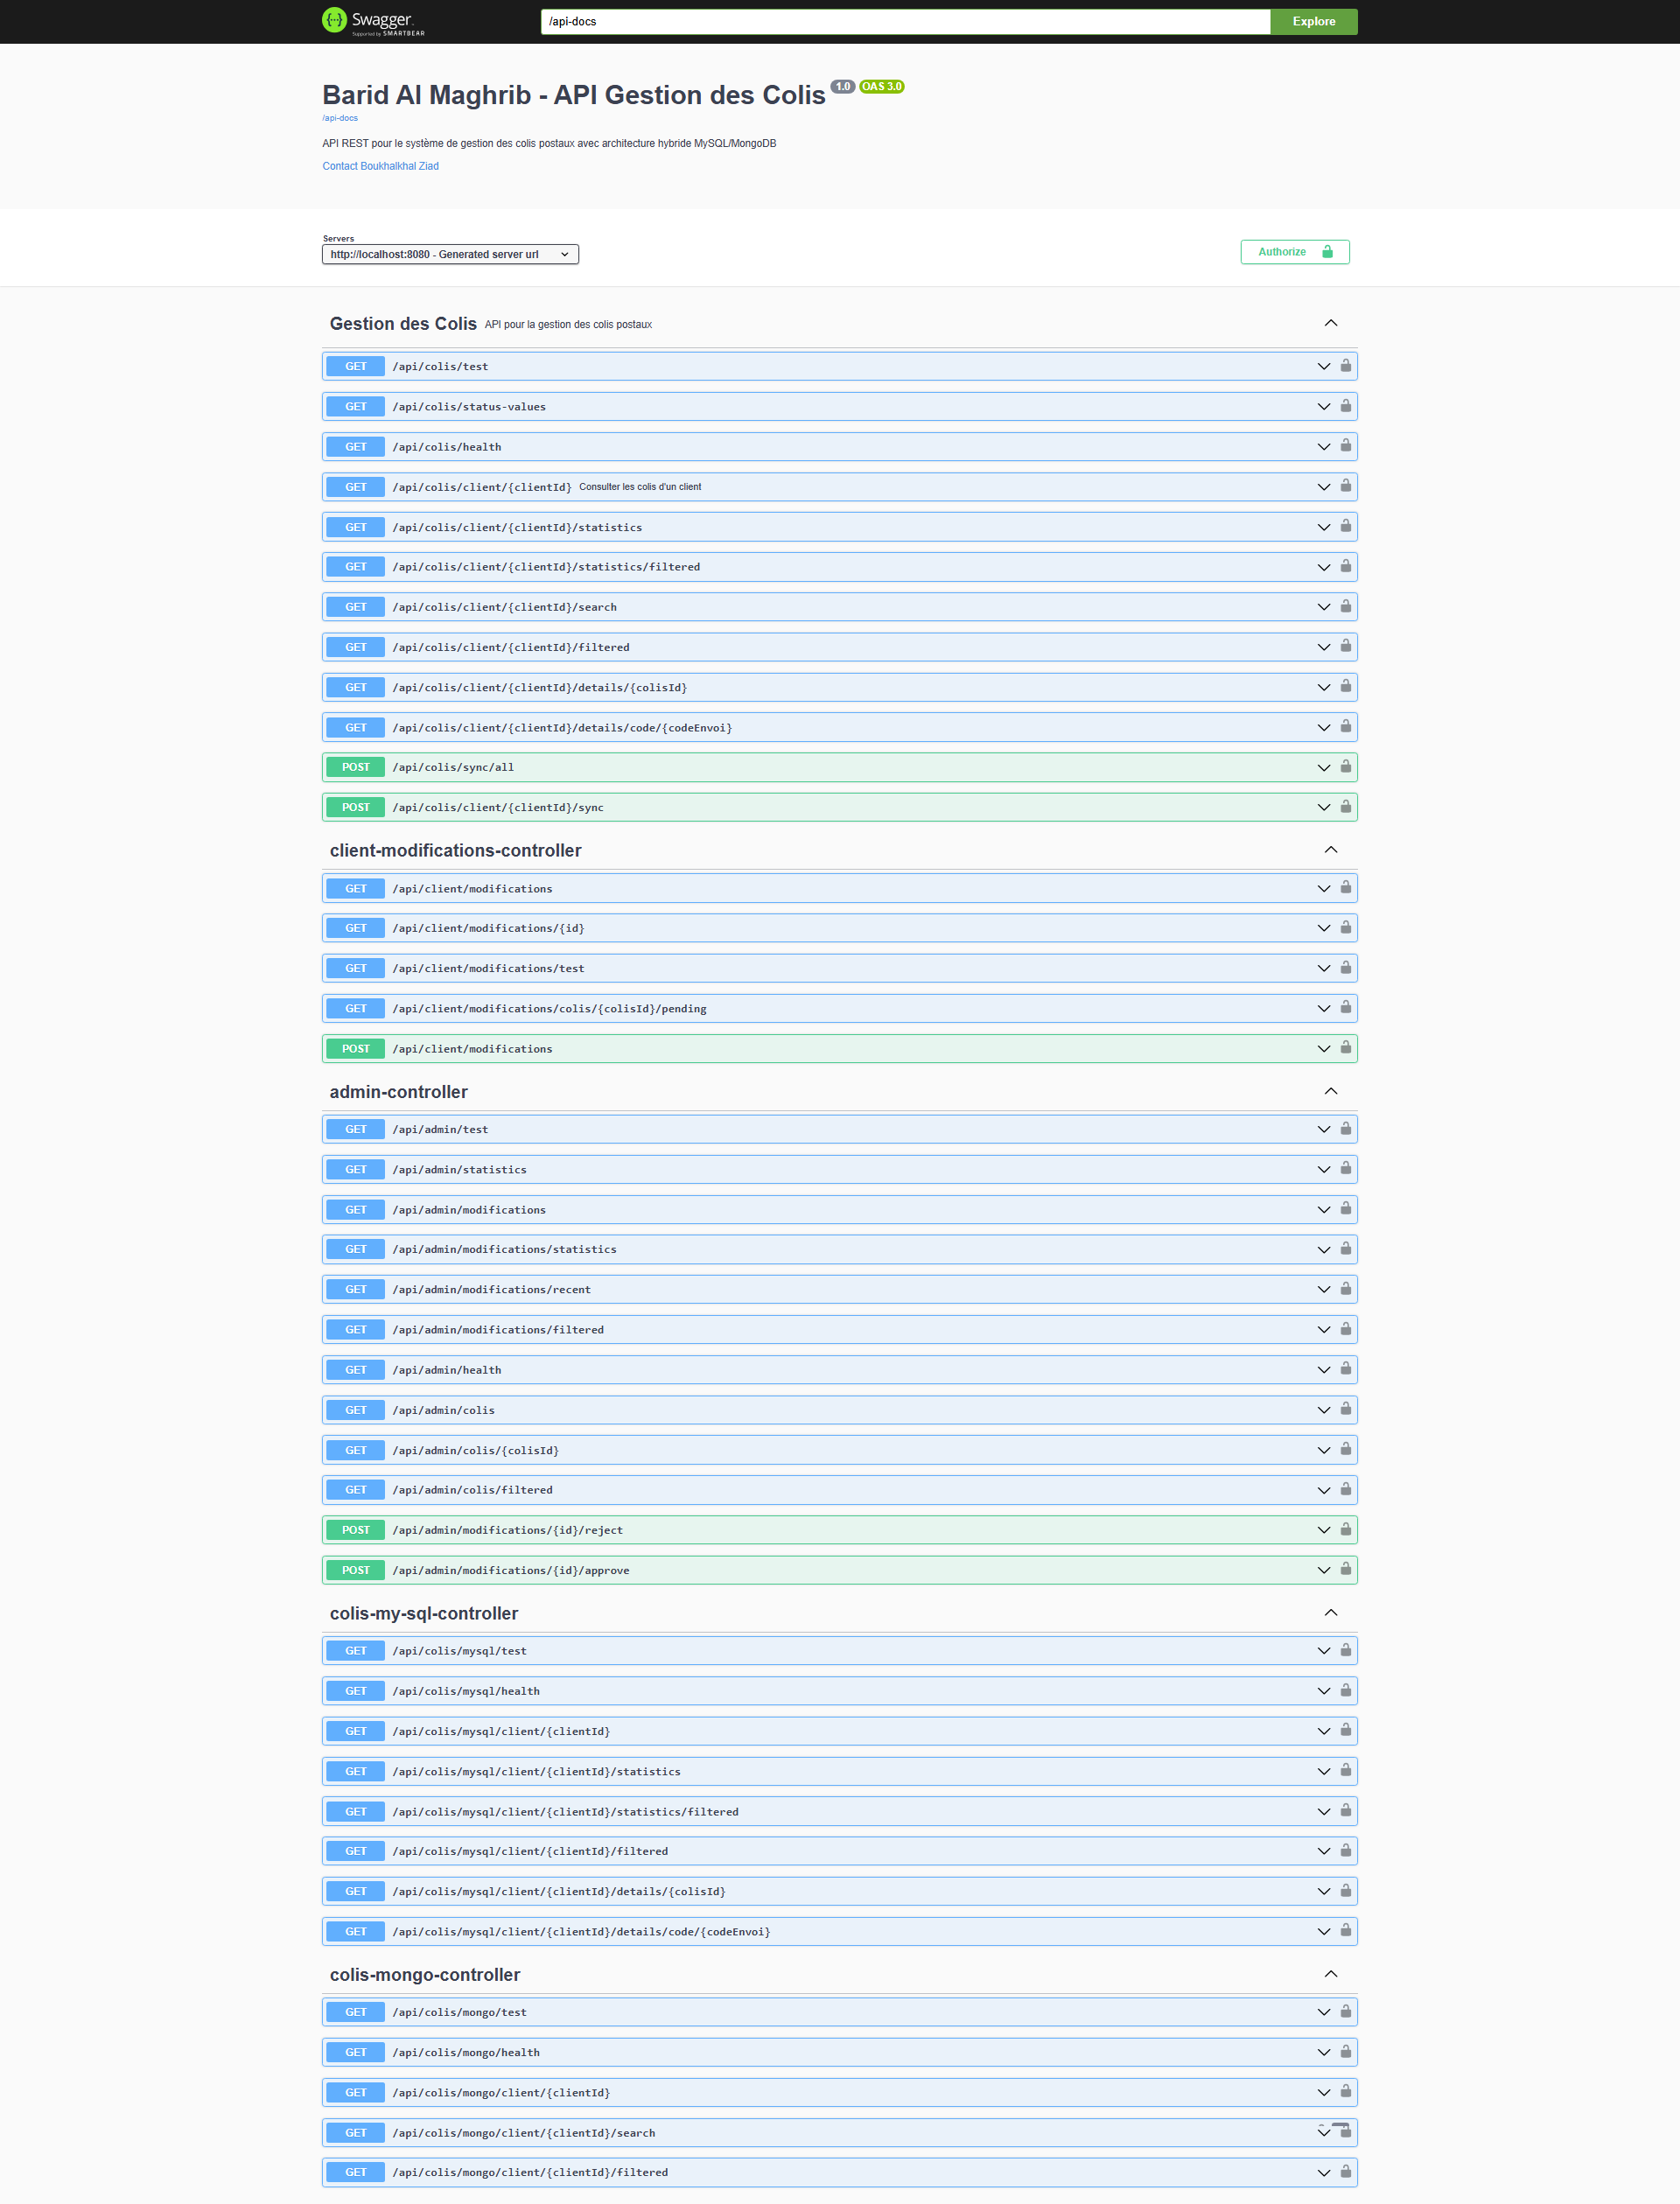
\includegraphics[width=0.7\textwidth]{images/api_endpoints.png}
\caption{Documentation des endpoints API REST}
\label{fig:api_endpoints}
\end{figure}

La Figure \ref{fig:api_endpoints} présente la documentation automatique des API REST générée par OpenAPI/Swagger. Les endpoints respectent les principes RESTful avec validation automatique des autorisations via l'extraction du \texttt{client\_id} depuis le token JWT. Chaque endpoint inclut la gestion d'erreurs appropriée et les codes de statut HTTP standards.

\subsection{Couche d'accès aux données}

L'implémentation du pattern Repository s'appuie sur Spring Data JPA pour MySQL et Spring Data MongoDB pour la base documentaire. Cette dualité nécessite une abstraction soignée pour masquer la complexité aux couches supérieures tout en exploitant les spécificités de chaque technologie.

\subsection{API REST}

\begin{figure}[H]
\centering
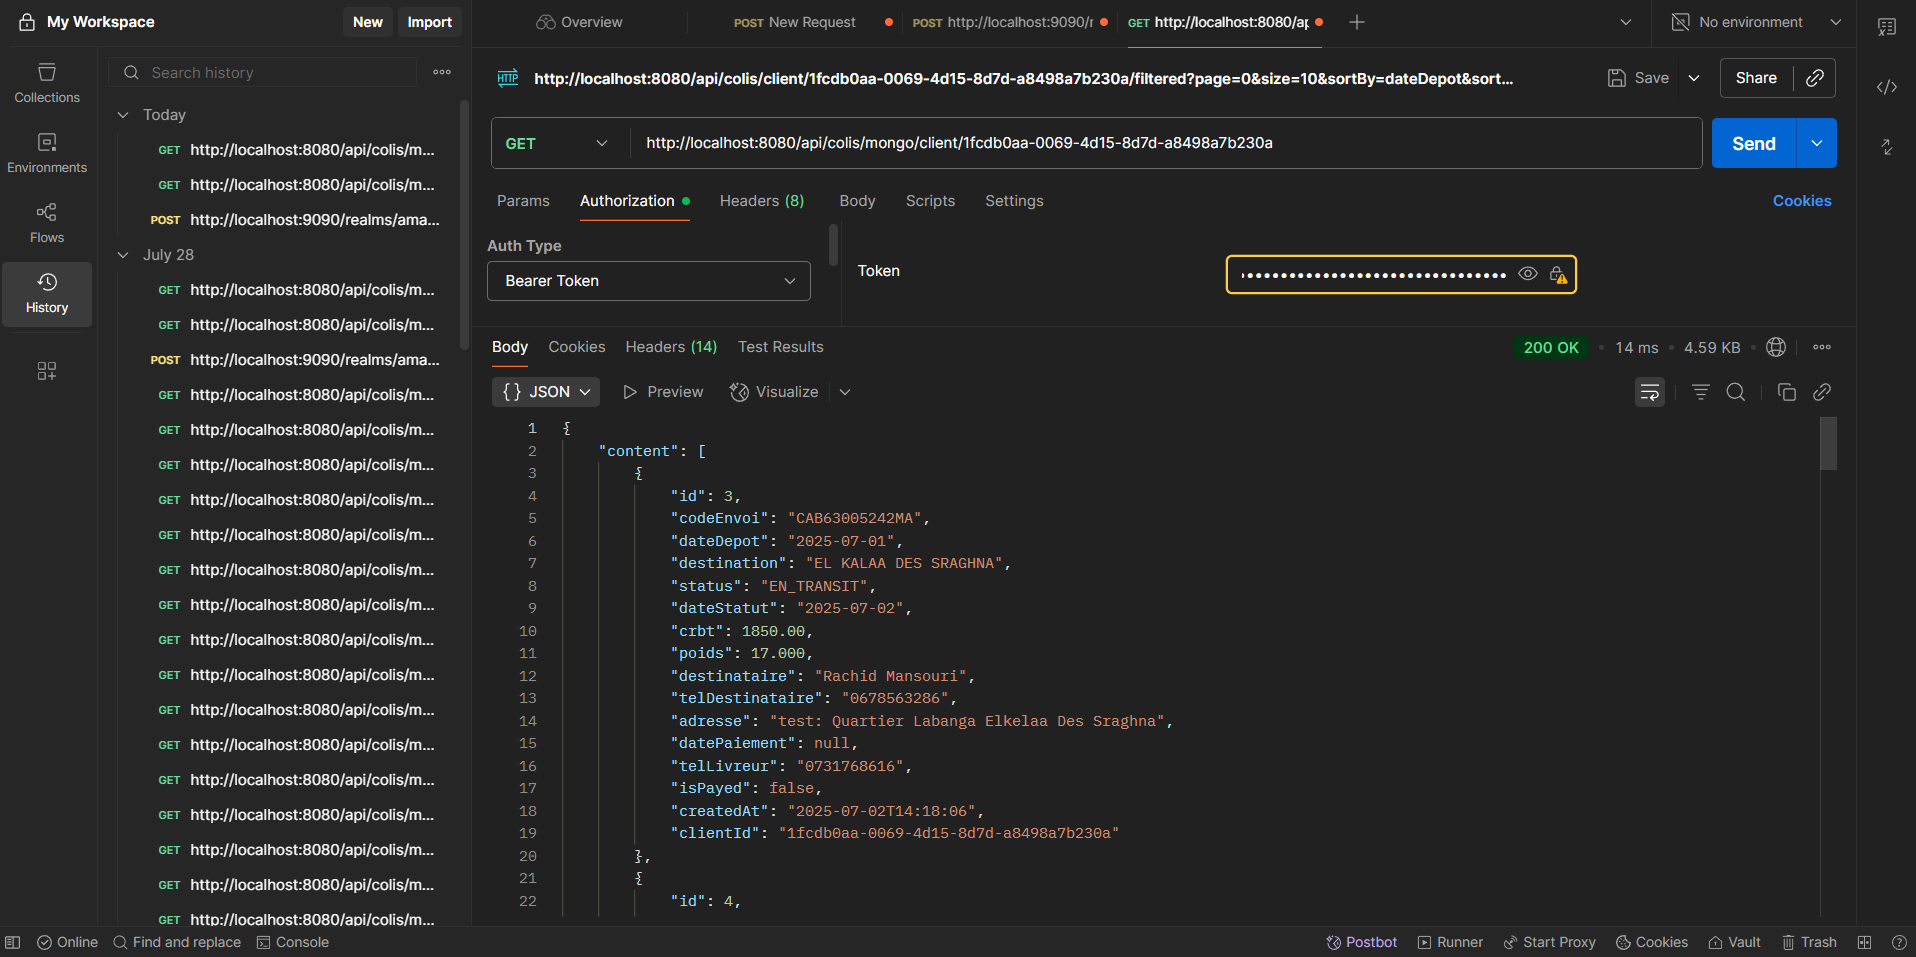
\includegraphics[width=1.0\textwidth]{images/postman_tests.png}
\caption{Tests des API avec Postman}
\label{fig:postman_tests}
\end{figure}

La Figure \ref{fig:postman_tests} montre les tests des API REST avec Postman [19], incluant la validation des tokens JWT [13], les tests de performance, et la vérification des autorisations. Cette approche garantit la robustesse et la sécurité des endpoints avant leur utilisation par le frontend.

\subsection{Sécurité avec Keycloak}

\begin{figure}[H]
\centering
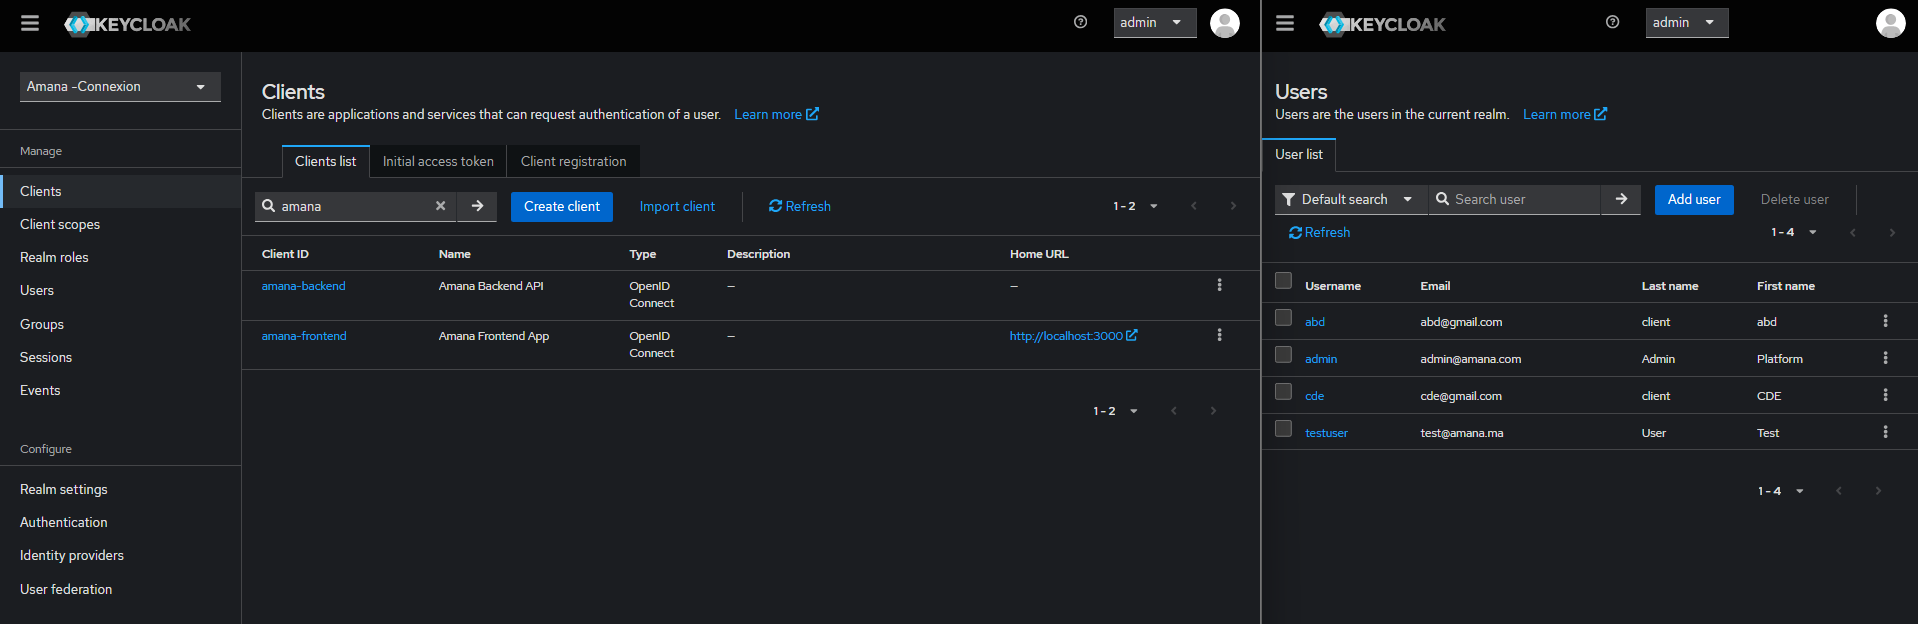
\includegraphics[width=1.0\textwidth]{images/keycloak_config.png}
\caption{Configuration Keycloak - Realm et clients}
\label{fig:keycloak_config}
\end{figure}

La Figure \ref{fig:keycloak_config} présente la configuration Keycloak avec le realm "amana-realm" et ses clients (backend et frontend). La configuration inclut les rôles utilisateur (ADMIN, CLIENT), les mappers de tokens, et les paramètres de sécurité. Cette configuration centralise l'authentification et l'autorisation pour tout le système.

\subsubsection{Gestion des rôles et permissions}

\begin{figure}[H]
\centering
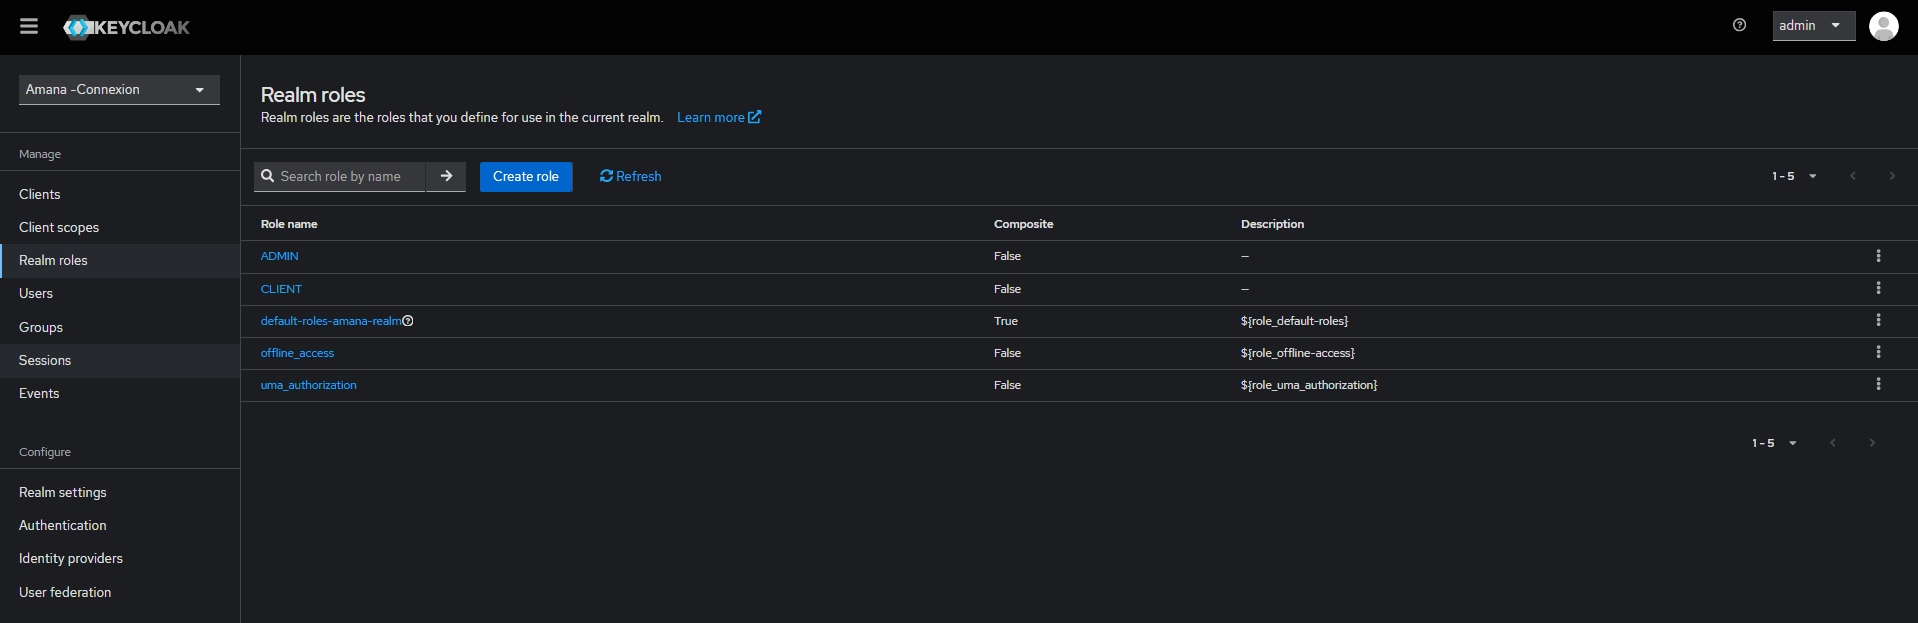
\includegraphics[width=0.8\textwidth]{images/keycloak_roles.png}
\caption{Gestion des rôles utilisateur dans Keycloak}
\label{fig:keycloak_roles}
\end{figure}

La Figure \ref{fig:keycloak_roles} détaille la gestion des rôles dans Keycloak. Les rôles CLIENT et ADMIN déterminent les autorisations d'accès aux données et fonctionnalités. Cette gestion fine des permissions garantit l'isolation des données clients et la sécurité globale du système.

\subsubsection{Protection des endpoints}

La protection des endpoints utilise Spring Security avec validation automatique des tokens JWT. Chaque requête est interceptée pour vérifier l'authenticité du token, extraire les informations utilisateur, et valider les autorisations d'accès aux ressources demandées.

\section{Intégration MongoDB}

\subsection{Configuration MongoDB}

\begin{figure}[H]
\centering
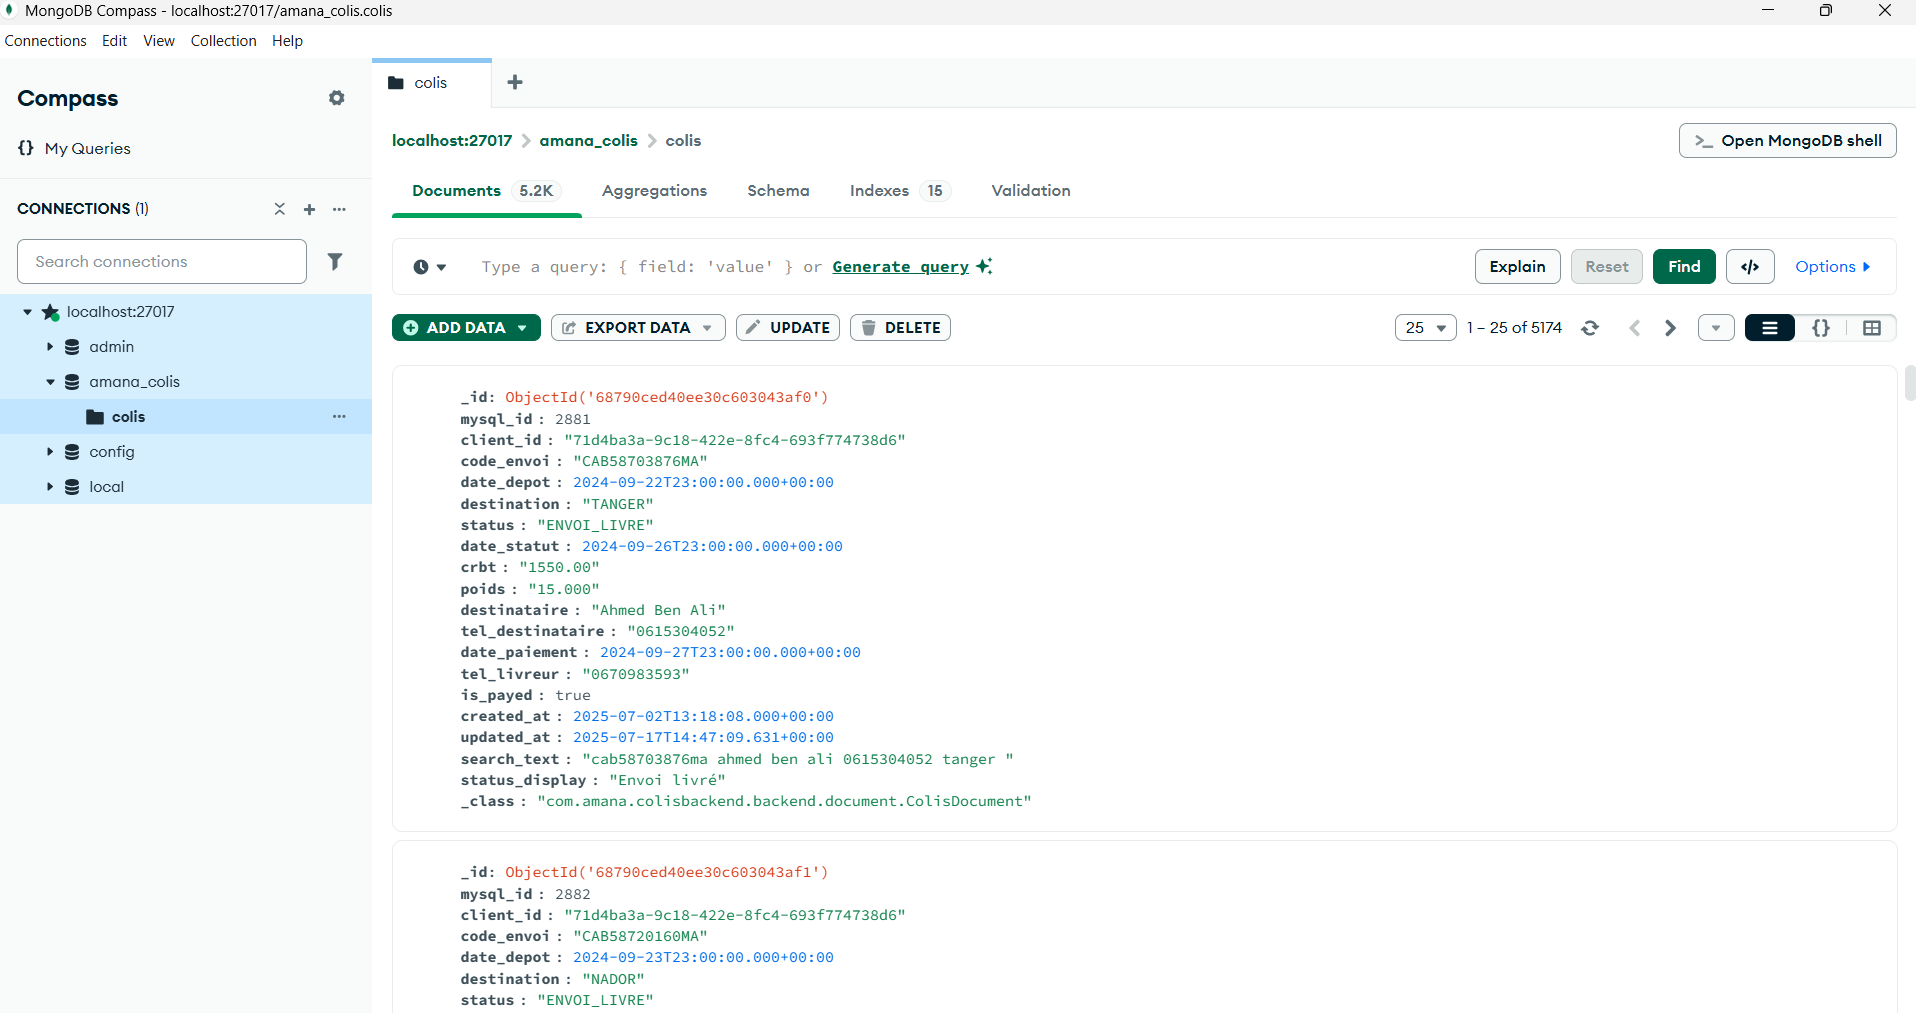
\includegraphics[width=1.0\textwidth]{images/mongodb_compass.png}
\caption{Interface MongoDB Compass - Gestion des collections}
\label{fig:mongodb_compass}
\end{figure}

La Figure \ref{fig:mongodb_compass} montre l'interface MongoDB Compass [20] utilisée pour la gestion et le monitoring de la base de données documentaire. L'outil permet de visualiser la structure des documents, gérer les index, et surveiller les performances des requêtes en temps réel.

\subsection{Modèles de documents}

La structure des documents MongoDB a été optimisée pour les performances de lecture avec des champs calculés et une dénormalisation appropriée. Les documents incluent les données métier essentielles ainsi que des champs optimisés pour la recherche et la visualisation.

\subsection{Repositories MongoDB}

\begin{figure}[H]
\centering
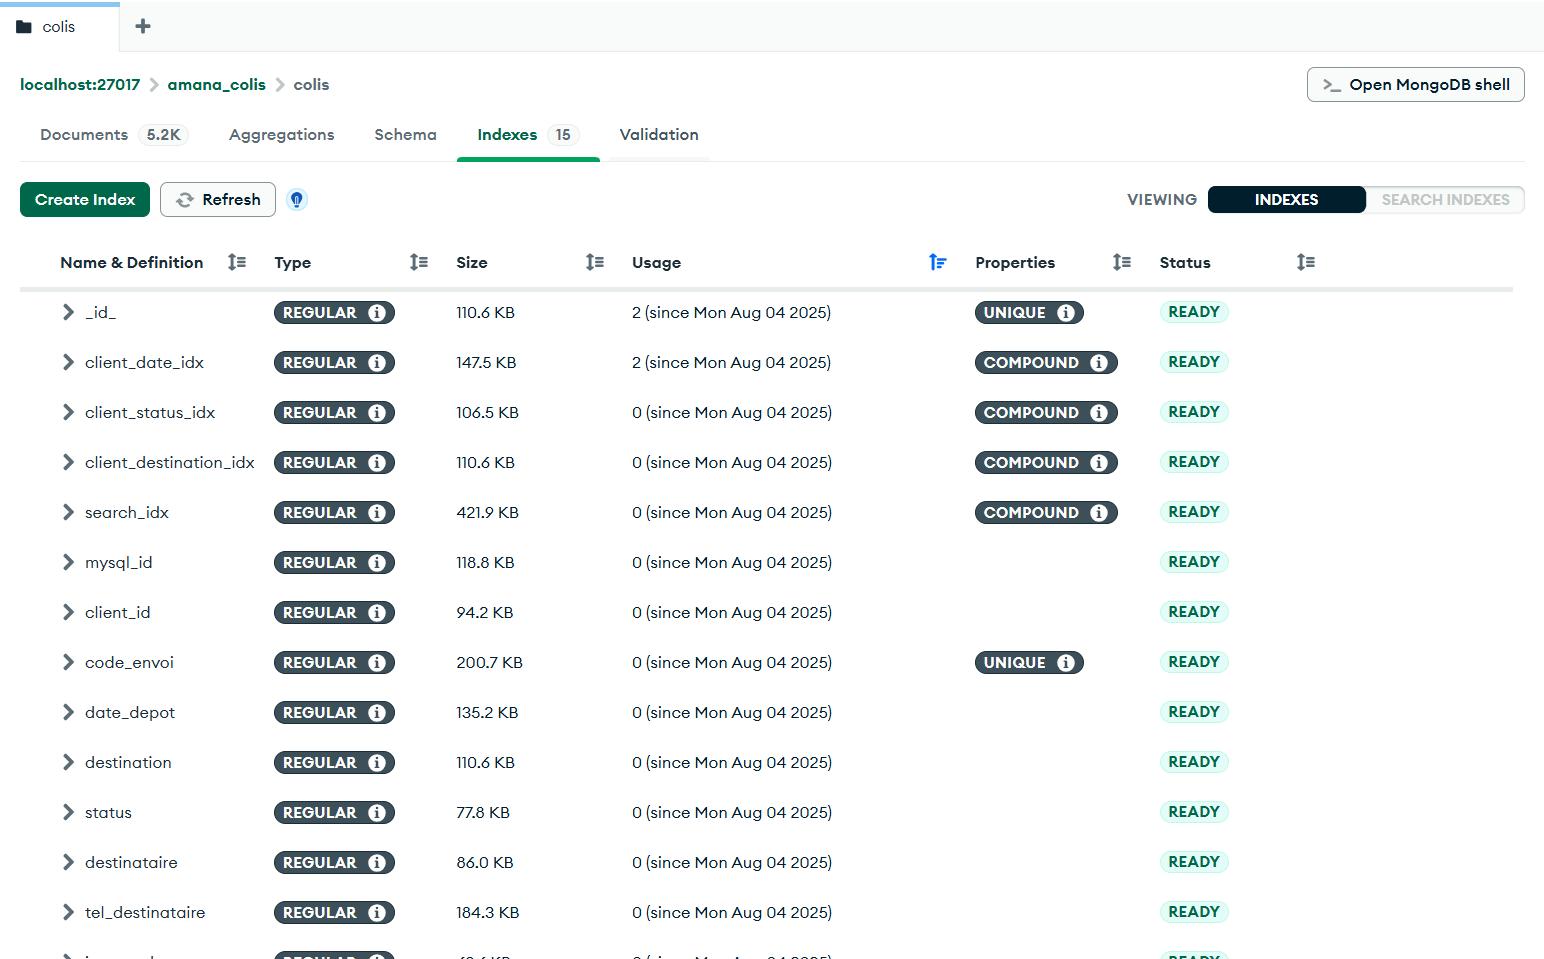
\includegraphics[width=1.0\textwidth]{images/mongodb_indexes.png}
\caption{Index MongoDB pour optimisation des performances}
\label{fig:mongodb_indexes}
\end{figure}

La Figure \ref{fig:mongodb_indexes} détaille la stratégie d'indexation MongoDB avec les index composés, textuels, et géospatiaux. Cette indexation spécialisée optimise les performances selon les patterns d'usage identifiés : consultation par client, recherche full-text, et requêtes géographiques.
\section{Développement Frontend}

\subsection{Interface utilisateur React}

\begin{figure}[H]
\centering
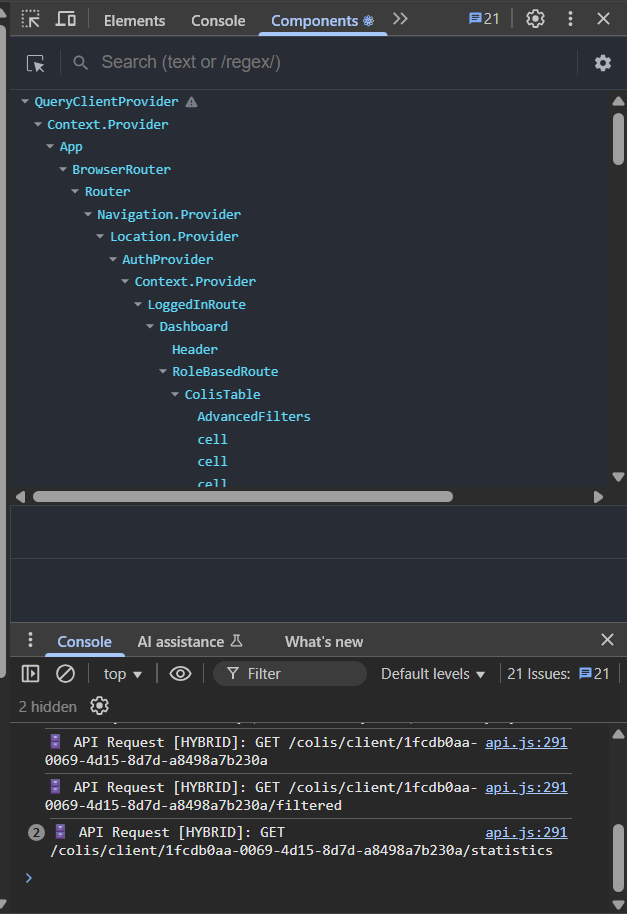
\includegraphics[width=0.7\textwidth]{images/react_dev_tools.png}
\caption{Développement React avec DevTools}
\label{fig:react_dev_tools}
\end{figure}

La Figure \ref{fig:react_dev_tools} montre l'environnement de développement React avec les DevTools permettant l'inspection des composants, la gestion des états, et le debugging des performances. Cette tooling avancée facilite le développement et l'optimisation de l'interface utilisateur.

\subsection{Intégration Keycloak Frontend}

\begin{figure}[H]
\centering
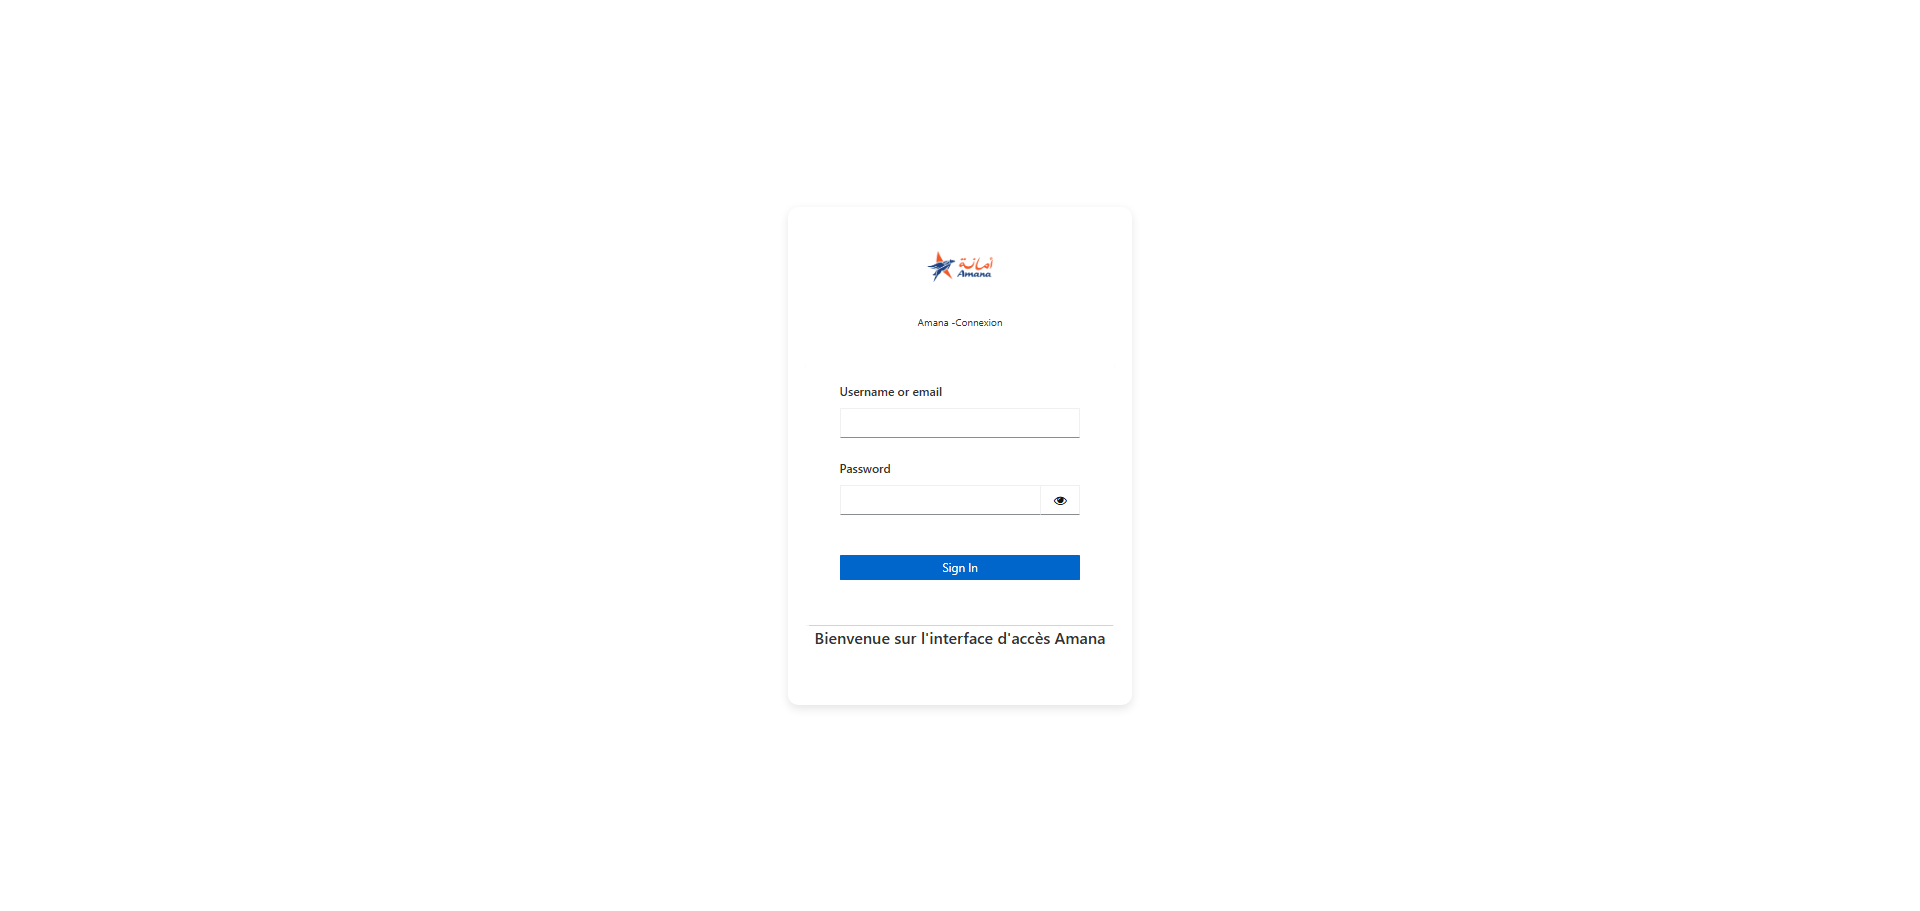
\includegraphics[width=0.7\textwidth]{images/keycloak_login.png}
\caption{Interface de connexion Keycloak}
\label{fig:keycloak_login}
\end{figure}

La Figure \ref{fig:keycloak_login} présente l'interface de connexion Keycloak intégrée dans l'application. Cette interface sécurisée gère l'authentification utilisateur avec support des standards OAuth 2.0 et OpenID Connect, offrant une expérience utilisateur fluide et sécurisée.

\subsection{Composants de visualisation}

L'architecture des composants React suit une approche modulaire avec séparation claire entre composants de présentation et composants containers. Cette organisation facilite la réutilisabilité, les tests, et la maintenance du code frontend.

\subsection{Intégration cartographique}

\begin{figure}[H]
\centering
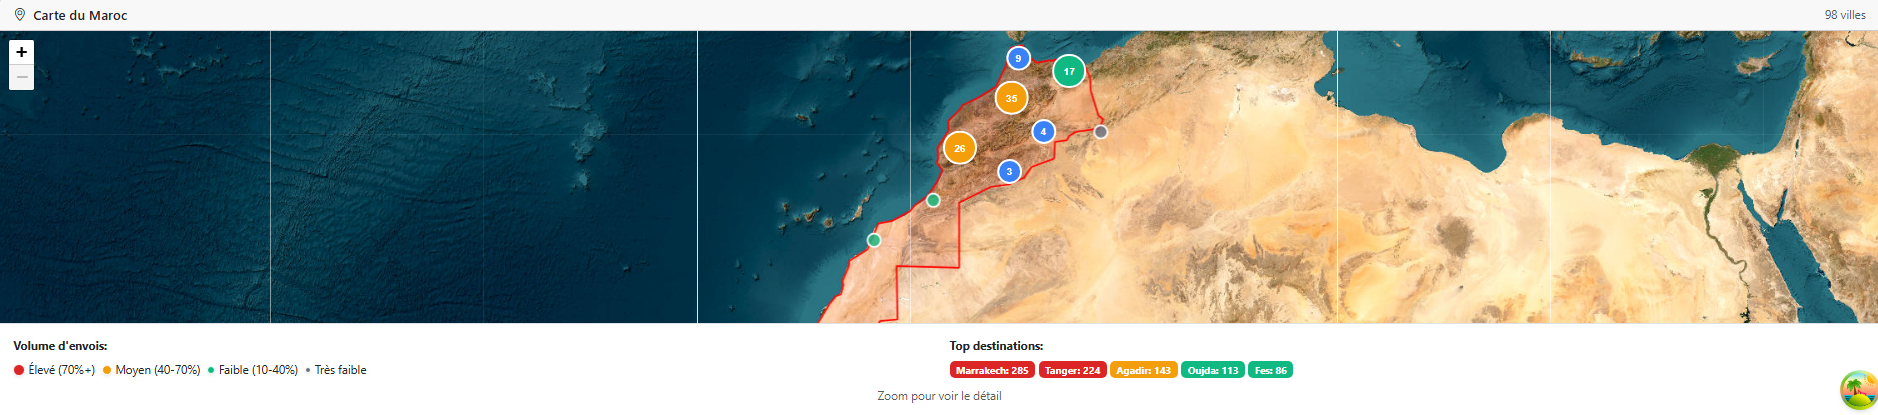
\includegraphics[width=1.0\textwidth]{images/leaflet_integration.png}
\caption{Intégration cartographique avec Leaflet}
\label{fig:leaflet_integration}
\end{figure}

La Figure \ref{fig:leaflet_integration} présente l'intégration cartographique utilisant Leaflet avec tiles haute résolution et clustering intelligent. Cette implémentation remplace l'affichage GeoJSON basique par une solution performante capable de gérer des milliers de points simultanément avec des performances optimales.

\subsection{Gestion des états}

La gestion des états utilise React Context pour les données globales (authentification, configuration) et useState/useEffect pour les états locaux des composants. Cette approche équilibrée évite la complexité excessive tout en maintenant la performance et la maintenabilité.

\section{Fonctionnalités Implémentées}

\subsection{Gestion des colis}

\begin{figure}[H]
\centering
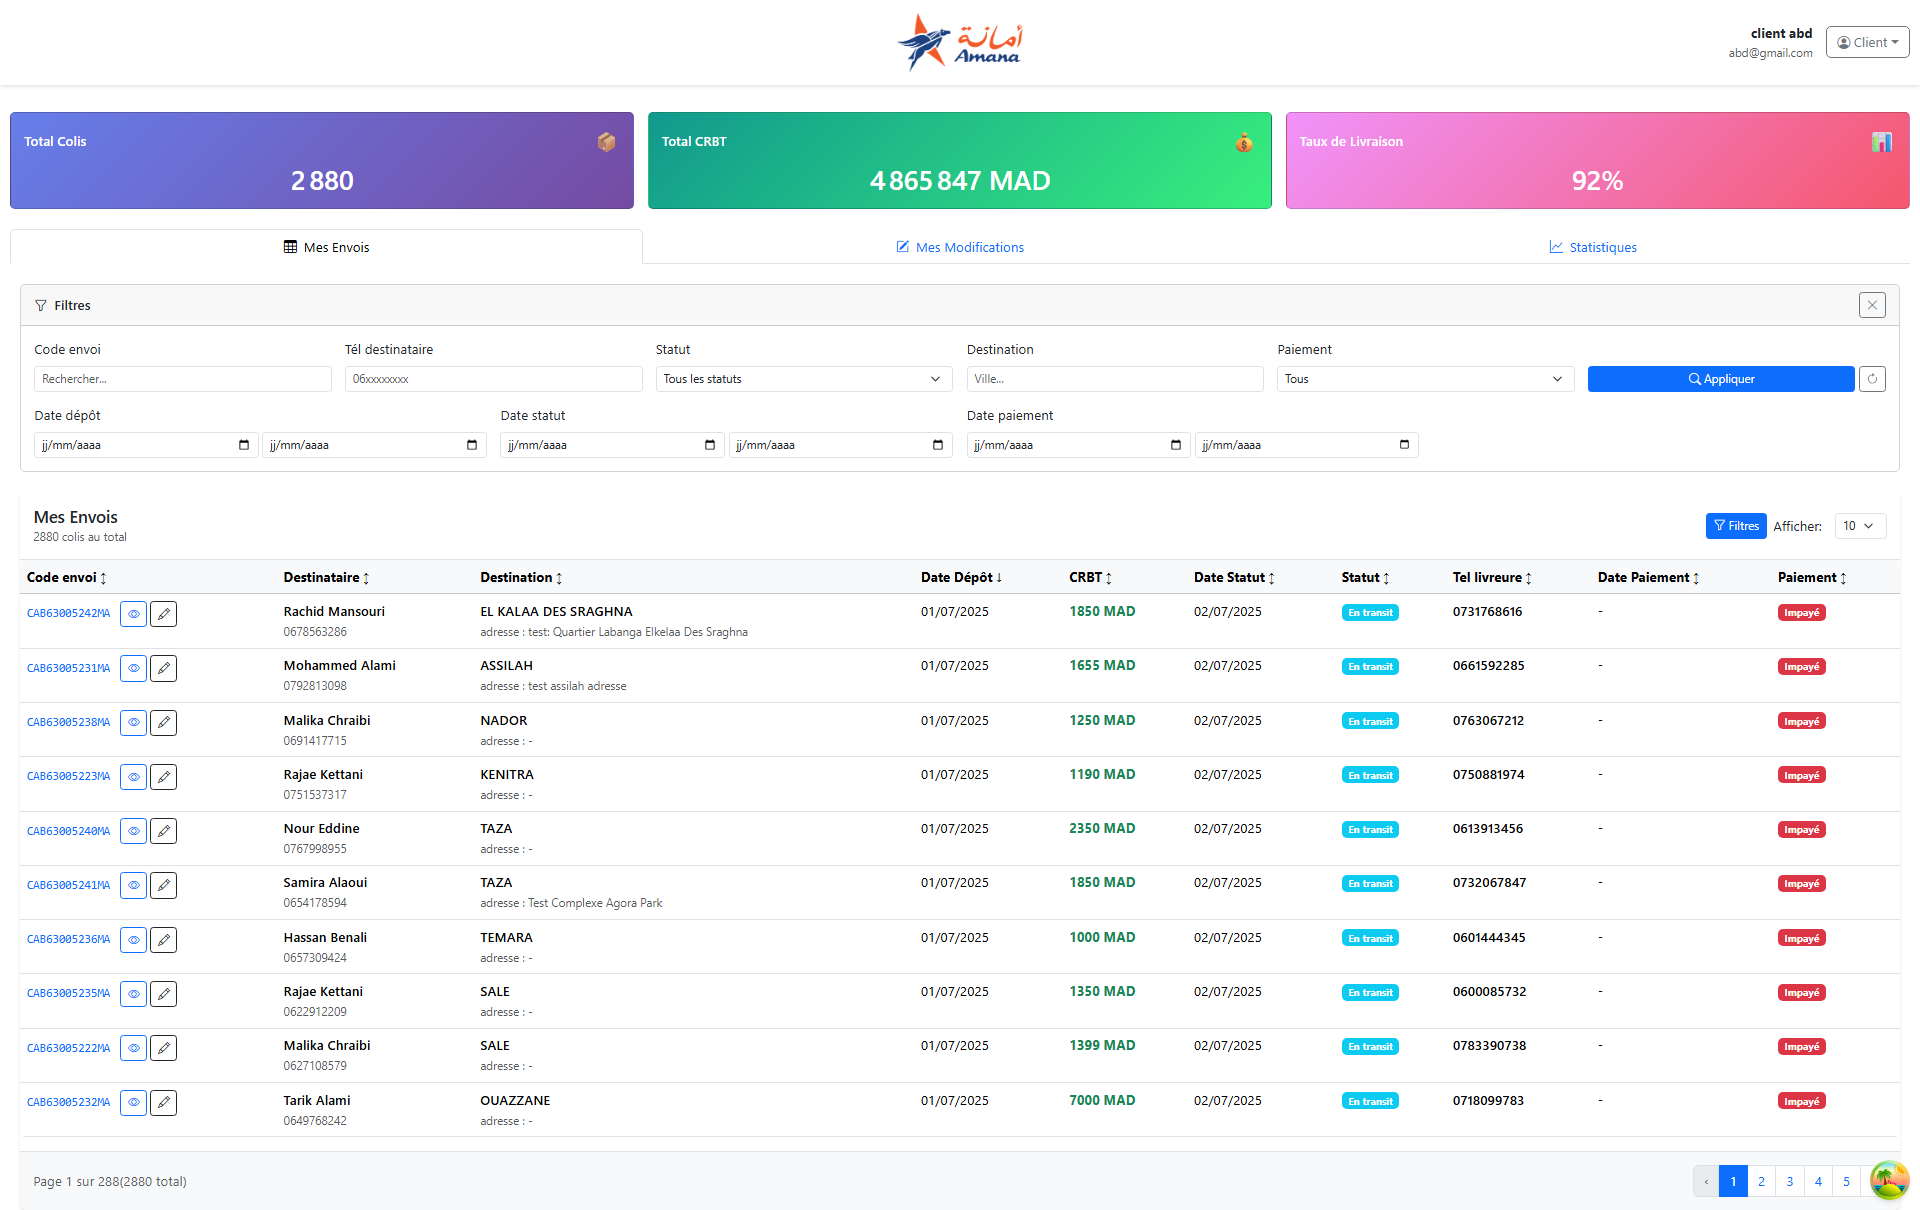
\includegraphics[width=1.0\textwidth]{images/colis_list_interface.png}
\caption{Interface de gestion des colis}
\label{fig:colis_list_interface}
\end{figure}

La Figure \ref{fig:colis_list_interface} montre l'interface principale de gestion des colis avec pagination optimisée, filtres avancés, et recherche intelligente. Cette interface exploite les performances MongoDB pour offrir une expérience utilisateur fluide même avec de gros volumes de données.

\subsection{Tableaux de bord}

\begin{figure}[H]
\centering
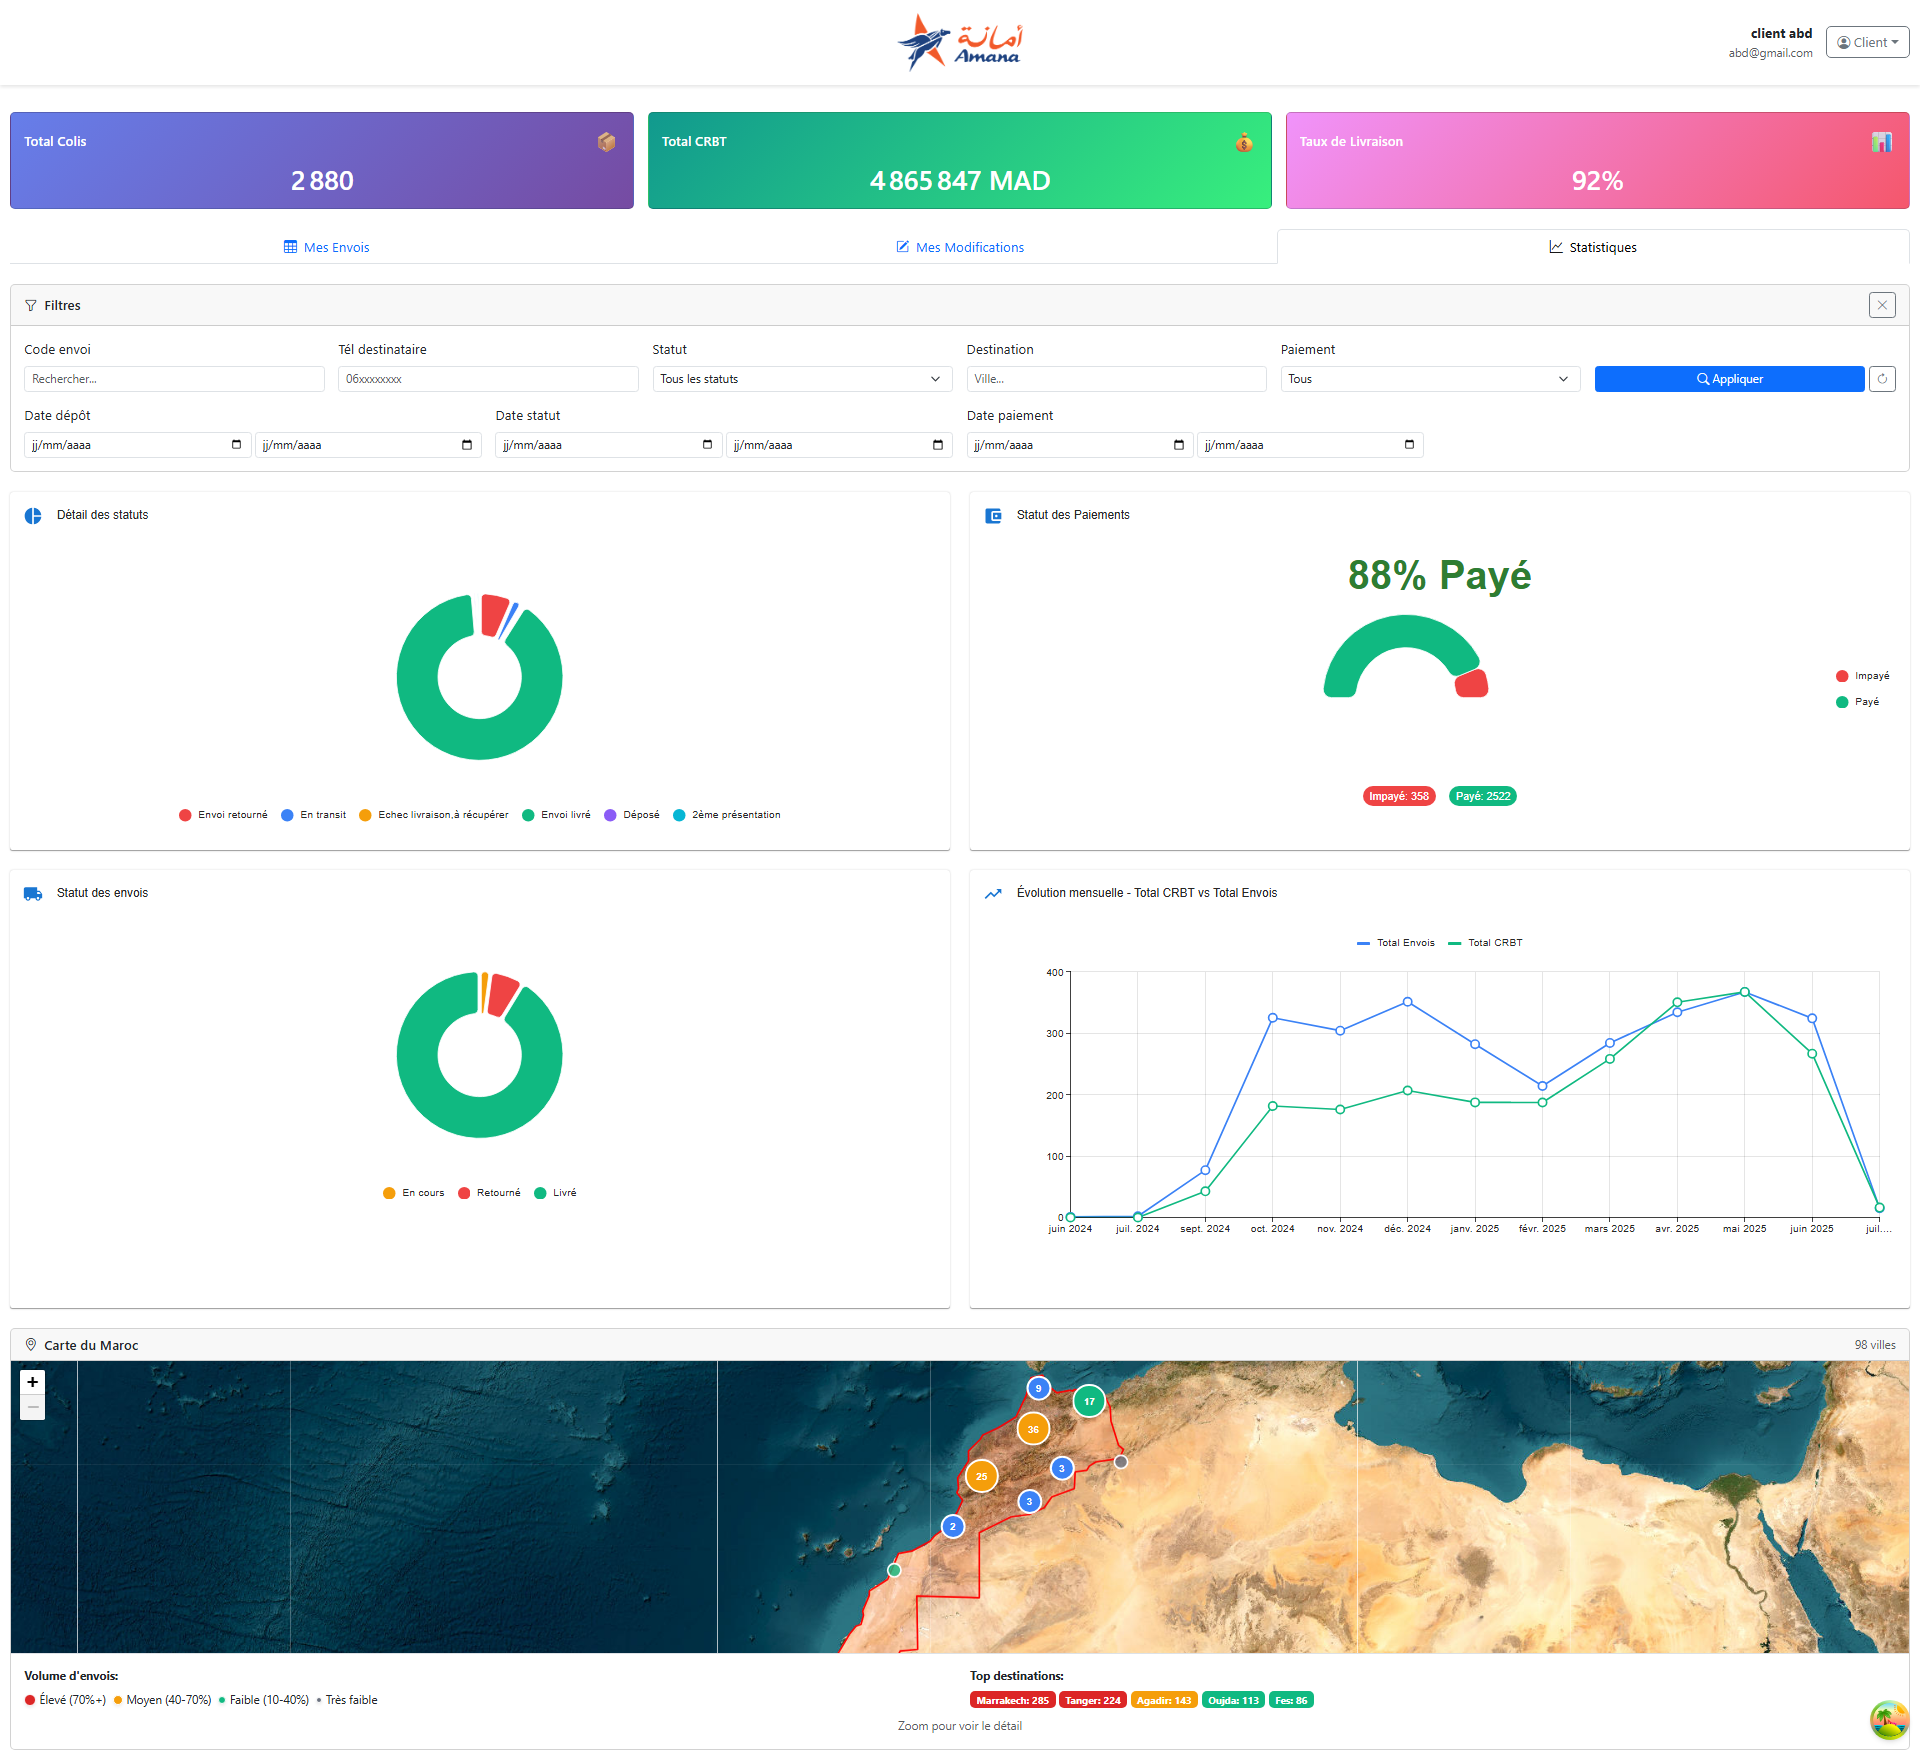
\includegraphics[width=1.0\textwidth]{images/dashboard_interface.png}
\caption{Tableaux de bord avec statistiques temps réel}
\label{fig:dashboard_interface}
\end{figure}

La Figure \ref{fig:dashboard_interface} illustre les tableaux de bord offrant une vue synthétique de l'activité avec graphiques interactifs et métriques en temps réel. Ces dashboards s'adaptent selon le profil utilisateur (client ou administrateur) pour présenter les informations pertinentes.

\subsection{Gestion des modifications}

\begin{figure}[H]
\centering
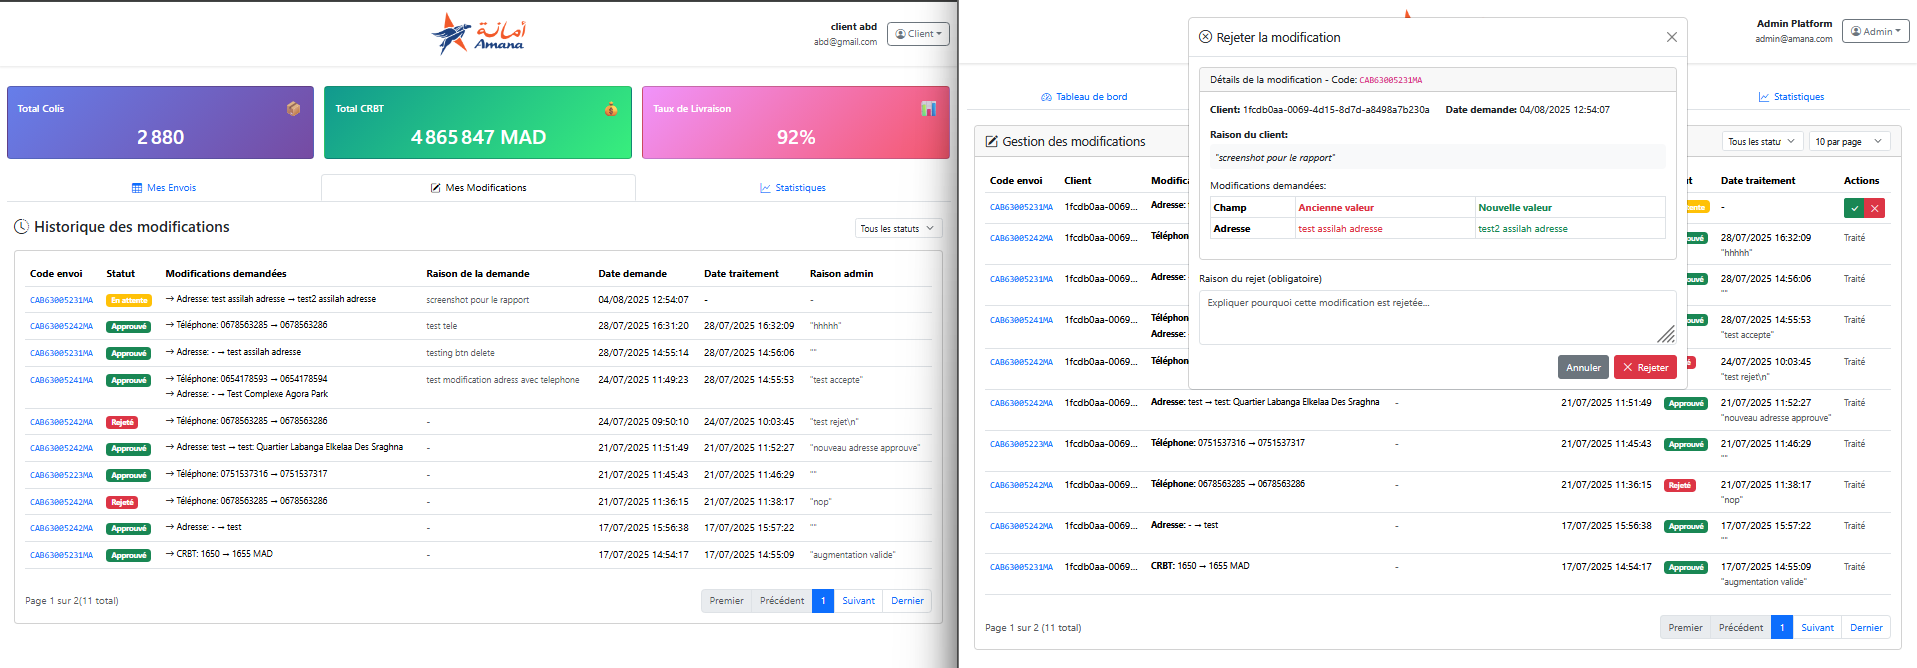
\includegraphics[width=1.0\textwidth]{images/modifications_workflow.png}
\caption{Interface de gestion des modifications - Workflow d'approbation}
\label{fig:modifications_workflow}
\end{figure}
La Figure \ref{fig:modifications_workflow} présente le système de gestion des demandes de modification avec workflow d'approbation. Cette interface permet aux clients de soumettre des demandes de changement et aux administrateurs de les valider ou rejeter avec traçabilité complète des actions effectuées.

\subsection{Interface administrateur}

\begin{figure}[H]
\centering
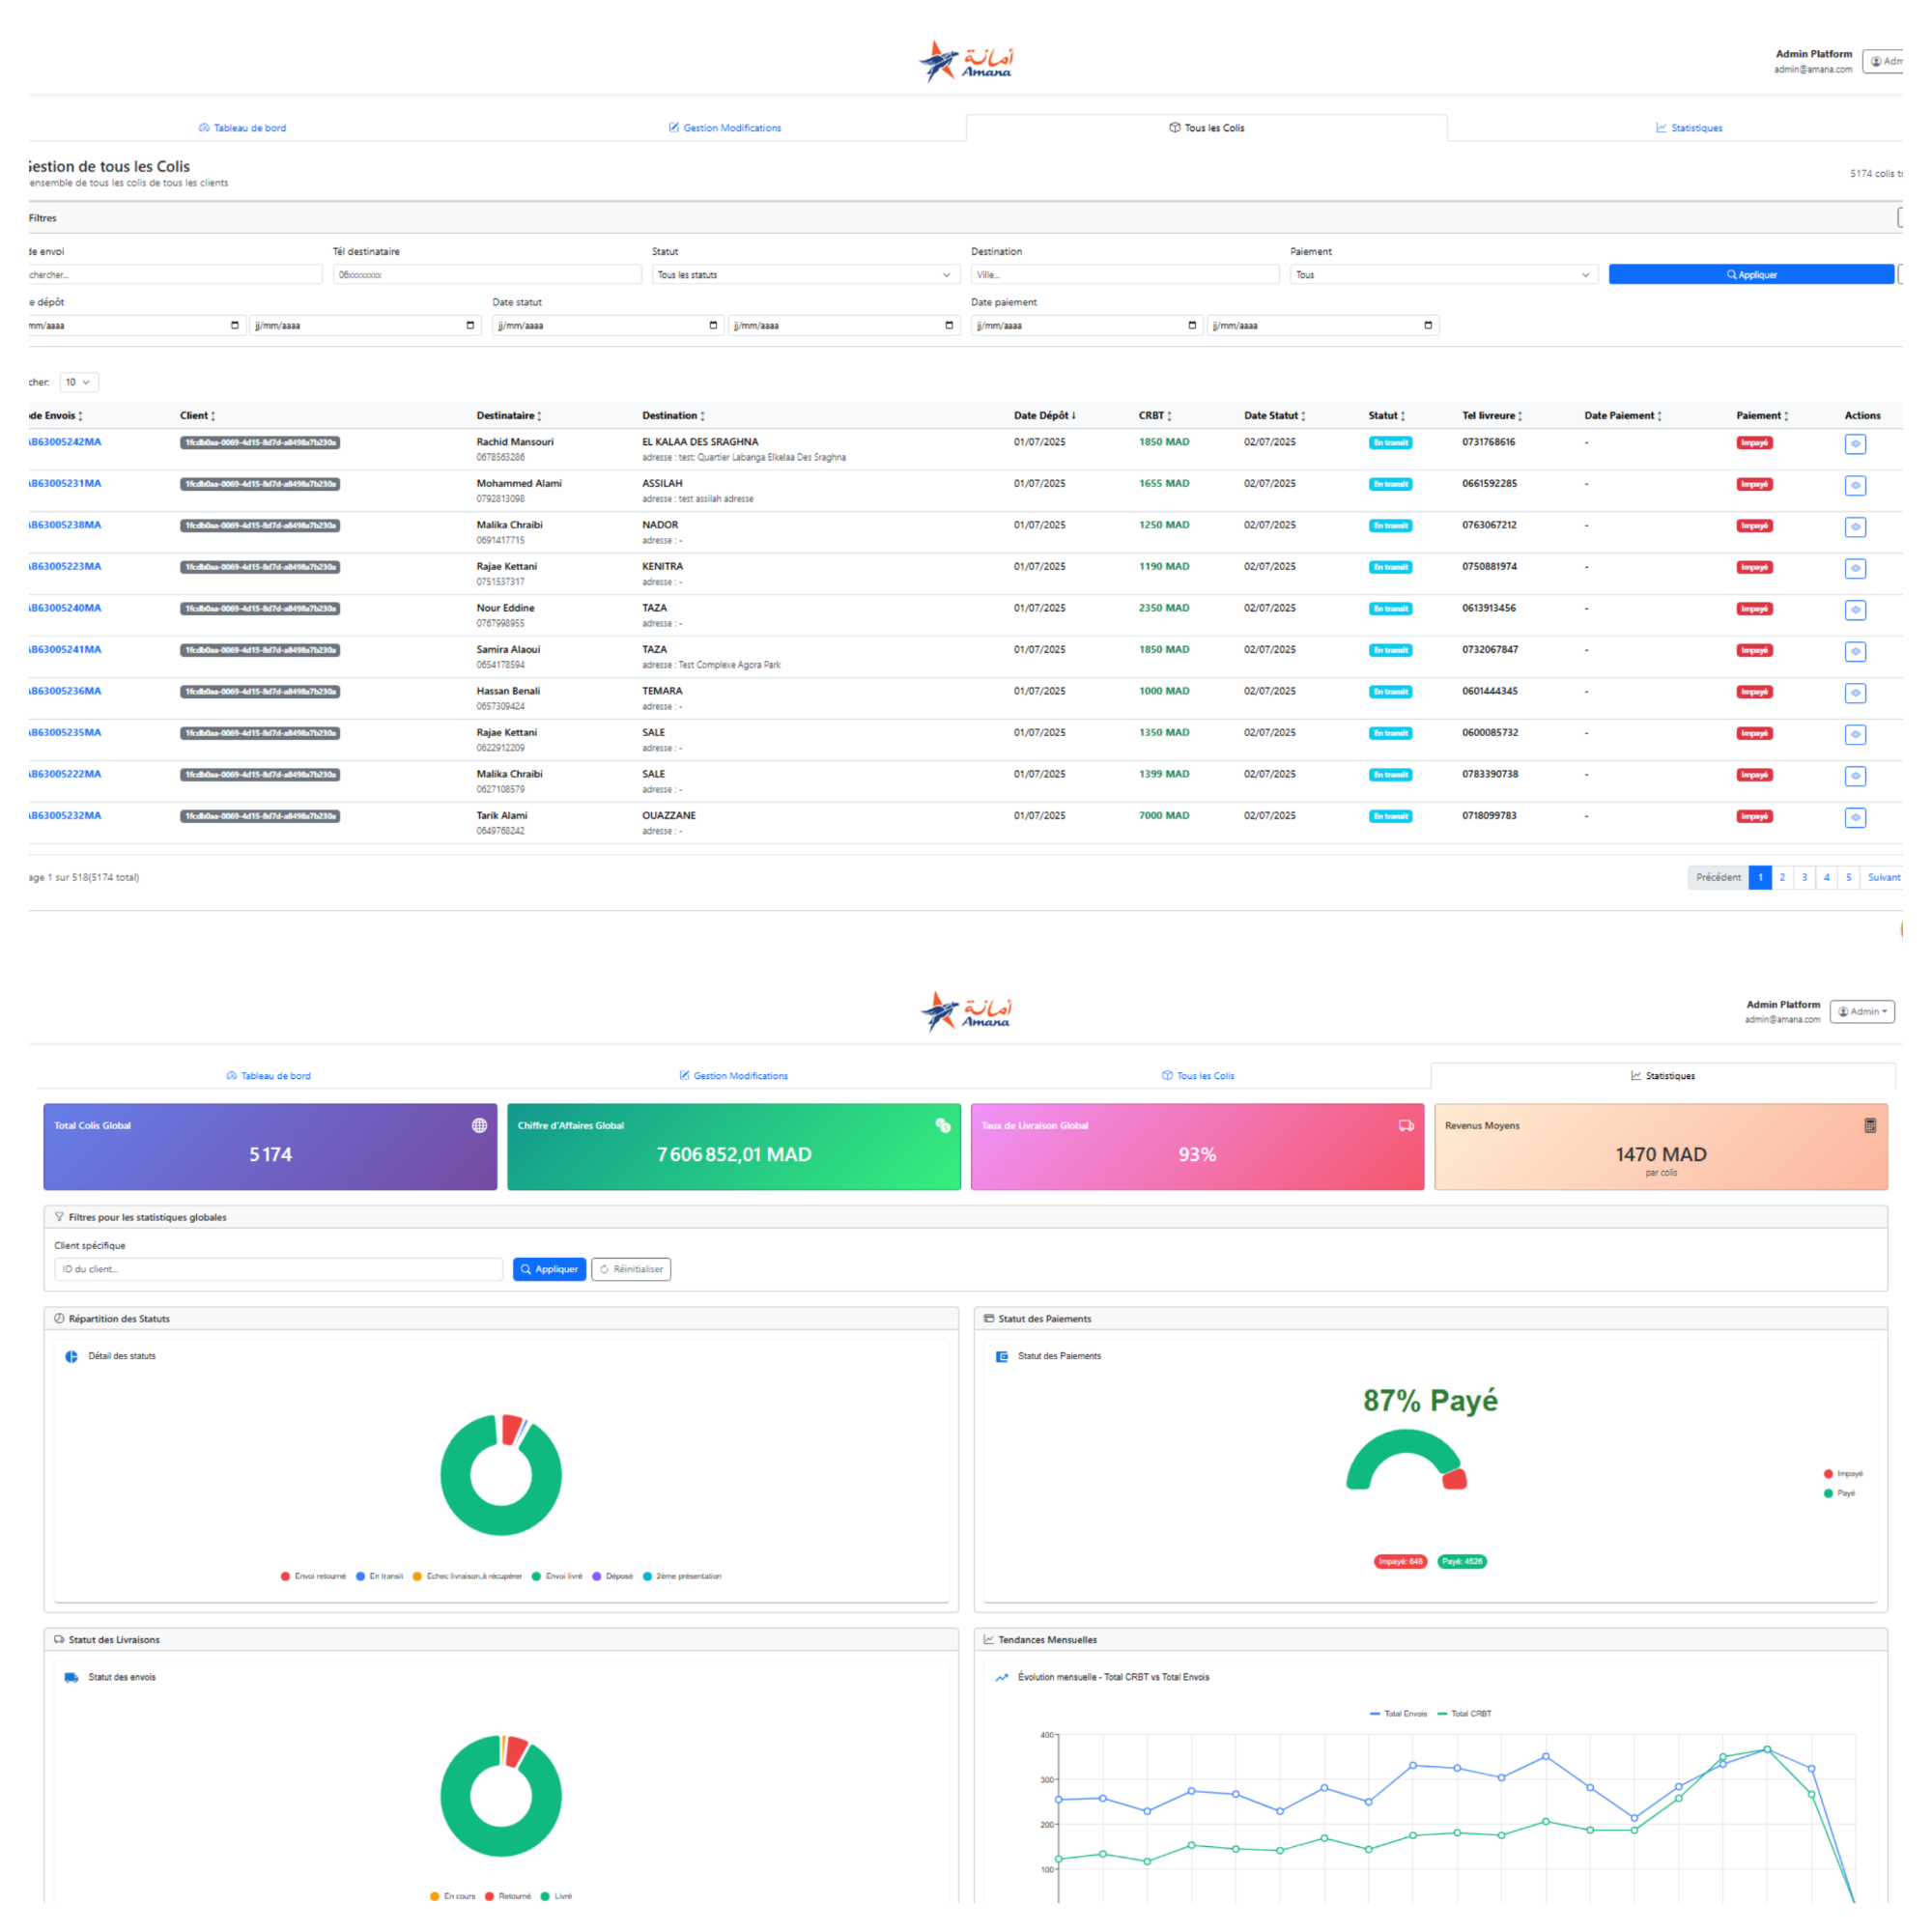
\includegraphics[width=0.6\textwidth]{images/admin_interface.png}
\caption{Interface administrateur - Vue globale du système}
\label{fig:admin_interface}
\end{figure}

La Figure \ref{fig:admin_interface} montre l'interface administrateur offrant une vue globale sur l'ensemble des données du système. Cette interface permet la supervision de tous les clients, la gestion des demandes de modification, et l'accès aux statistiques globales de performance.